\hypertarget{bonjour-monde}{%
\section{Bonjour, monde !}\label{bonjour-monde}}

\emph{Mardi 24 avril 2018}

Bonjour à tous !

Nous avons le plaisir de dévoiler au monde notre blog, destiné à
héberger les souvenirs à venir de notre voyage. Décollage prévu : 3 mai
2018.

\begin{figure}
\centering
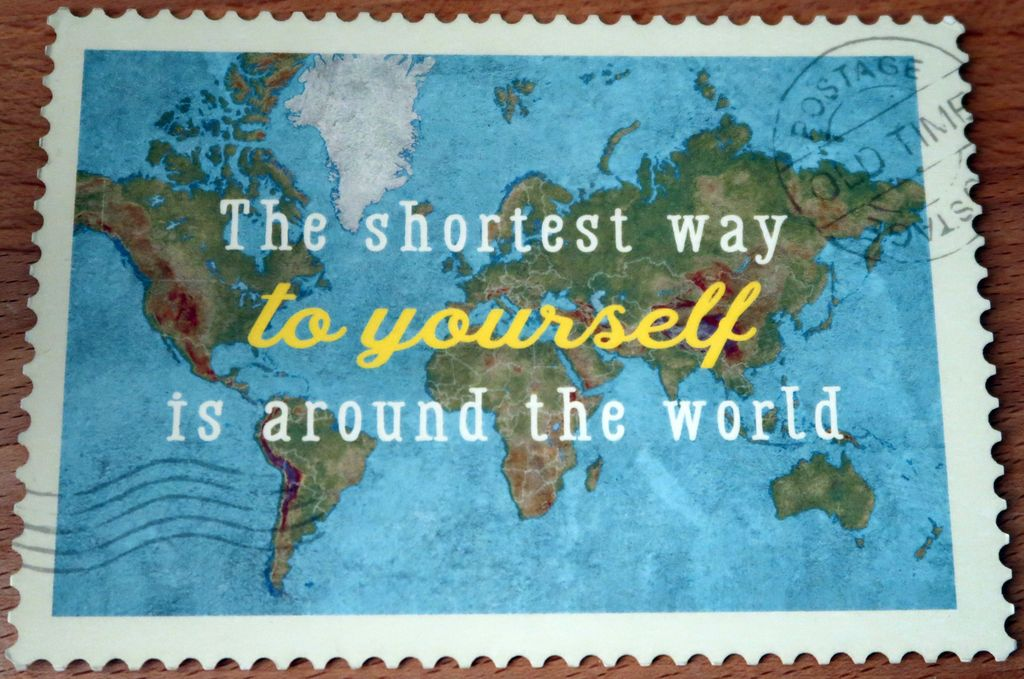
\includegraphics{images/world_postcard.jpg}
\caption{Merci à Marie-Christine pour cette carte postale qui incarne à
merveille l'esprit du voyage...}
\end{figure}

D'ici là, on vous laisse avec deux belles citations avant d'entamer
notre voyage à travers l'espace et à travers le temps :

\begin{quote}
Nous n'aurons de cesse d'explorer et la fin de toutes nos explorations
sera de revenir à l'endroit d'où nous sommes partis et de connaître le
lieu pour la première fois.
\end{quote}

\emph{T. S. Eliot, cité par Jean Claude Ameisen}

\begin{quote}
"Vous avez longtemps voyagé", dit le Simurgh à ses sujets les oiseaux,
lorsqu'ils le découvrent enfin après une très longue quête, "vous avez
cru parfois vous perdre, mais vous ne vous êtes pas quittés. C'est vous
que vous avez retrouvés."
\end{quote}

\emph{Mantiq at-Tayr (La conférence des oiseaux), Farid Al-Din Attar cité par Jean Claude Ameisen}

\emph{Elida et Florian}

\hypertarget{commentaires}{%
\subsection{Commentaires}\label{commentaires}}

\begin{itemize}
\item
  kje, \emph{2018-05-03 13h59}

  Un conseil : laissez tomber les citations de citations d'obscurs
  ornithologues qui n'intéressent que l'élite germanopratine dont
  Florian est la coqueluche. Si vous voulez qu'on lise votre blog avec
  plus d'entrain que les mails de Sarah Dobigny sur l'avancement des
  travaux à nanoInnov, donnez-nous votre opinion sur le hezbollah ou
  parlez-nous de l'évolution du marché de l'emploi sur l'île de
  Paques... Soyez disruptifs...
\item
  Florian LB, \emph{2018-05-04 08h48}

  Cher KJE, merci pour cet encouragement qui va sans aucun doute nous
  tirer vers le haut (pas comme les ornithologues du XIIème siècle hein,
  tu as bien raison). Etant donné qu'on vient juste d'arriver au Liban,
  je ne peux pas encore te parler avec confiance du Hezbollah, mais les
  élections de ce week-end nous donneront, je l'espère, de quoi assouvir
  tes envies de news disruptives. On te tient au jus.
\end{itemize}
